\section{Question 2}\label{question-2}

\subsection{Inserting 2}

We convert it to binary \textit{010} and it should be placed to \textbf{Bucket C}. This is shown in Figure~\ref{fig:q2-1}.

\begin{figure}[H]
  \centering
  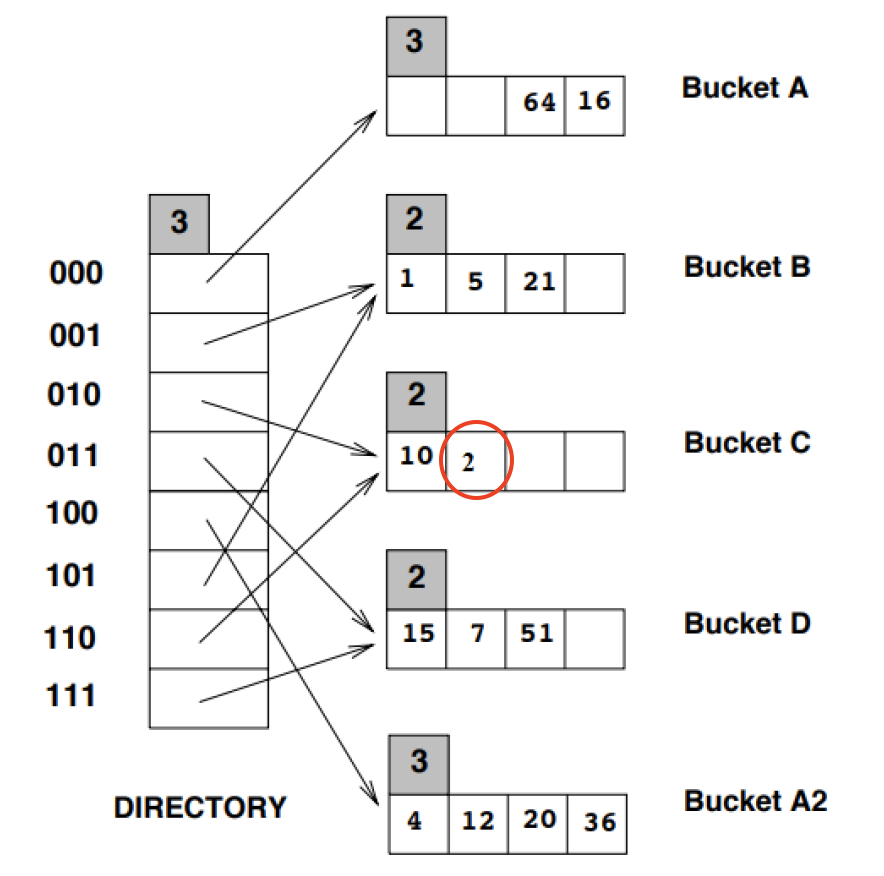
\includegraphics[width=0.9\linewidth]{figs/q2-1.png}
  \caption{Hash index after inserting 2}
  \label{fig:q2-1}
\end{figure}

\subsection{Inserting 25}

Similarly, its binary value is \textit{11001} and should be placed to \textbf{Bucket B}. This is shown in Figure~\ref{fig:q2-2}.

\begin{figure}[H]
  \centering
  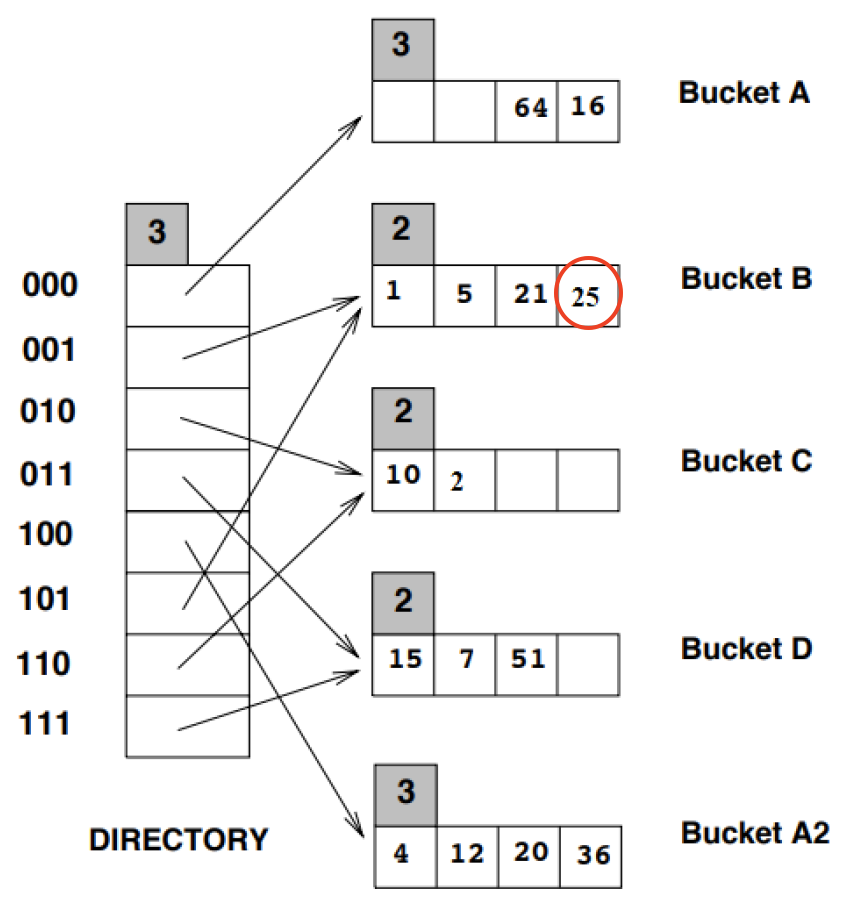
\includegraphics[width=0.9\linewidth]{figs/q2-2.png}
  \caption{Hash index after inserting 25}
  \label{fig:q2-2}
\end{figure}

\subsection{Inserting 0}

Similarly, its binary value is \textit{000} and should be placed to \textbf{Bucket A}.
This is shown in Figure~\ref{fig:q2-3}.

\begin{figure}[H]
  \centering
  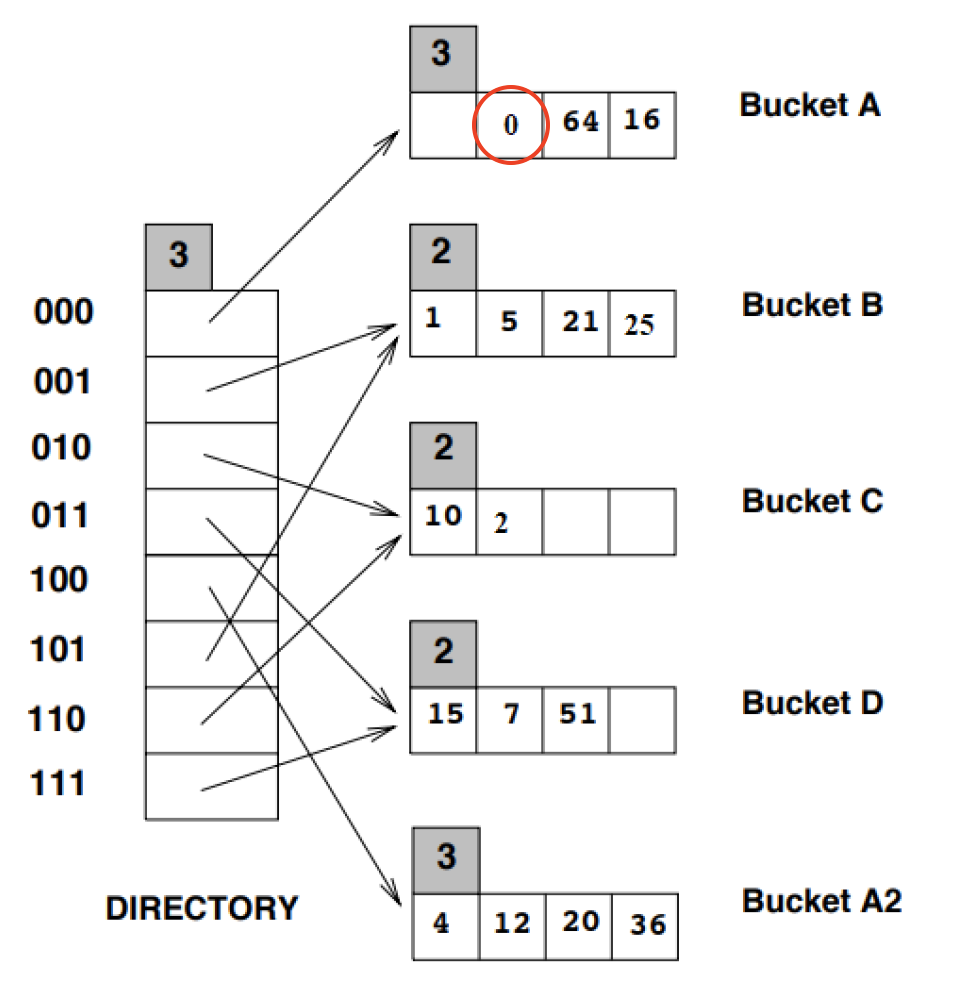
\includegraphics[width=0.9\linewidth]{figs/q2-3.png}
  \caption{Hash index after inserting 0}
  \label{fig:q2-3}
\end{figure}

\subsection{Inserting 31}

Similarly, its binary value is \textit{11111} and should be placed to \textbf{Bucket D}.
This is shown in Figure~\ref{fig:q2-4}.

\begin{figure}[H]
  \centering
  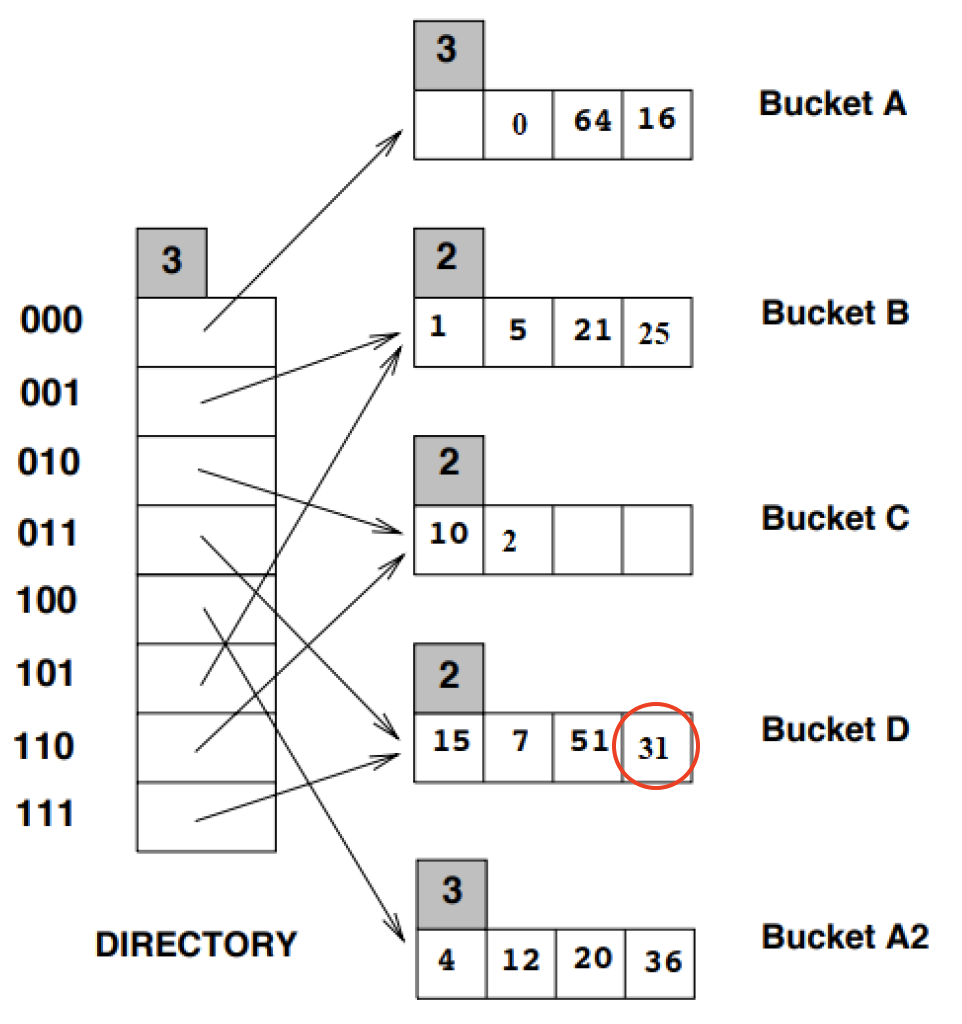
\includegraphics[width=0.9\linewidth]{figs/q2-4.png}
  \caption{Hash index after inserting 31}
  \label{fig:q2-4}
\end{figure}

\subsection{Inserting 68}

Finally, we need to split the bucket \textbf{A2} as there is no enough space for 68.
As a result, the new buckets have local depth 4 and The global depth is increased as well (now we take four least significant bits from binary numbers).
This is shown in Figure~\ref{fig:q2-5}.

\begin{figure}[H]
  \centering
  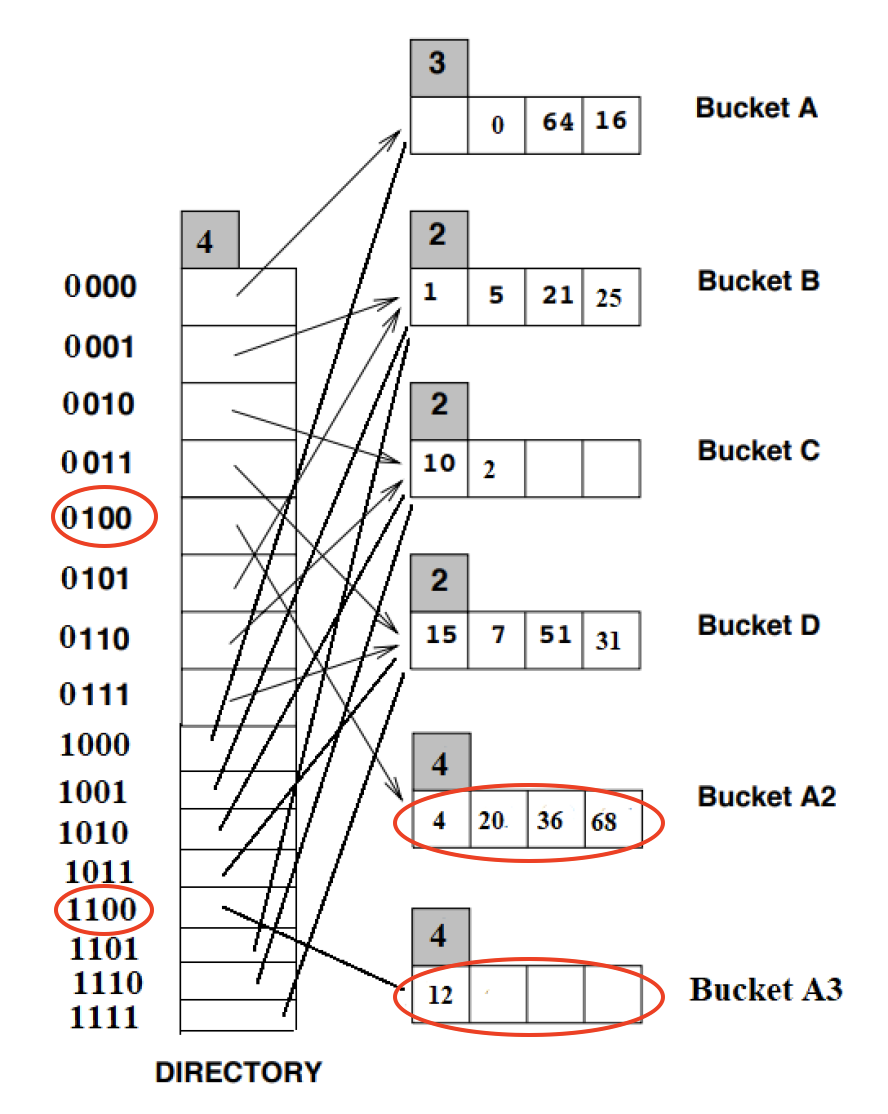
\includegraphics[width=0.9\linewidth]{figs/q2-5.png}
  \caption{Hash index after inserting 68.
    Bucket A2 is split into A2 and A3.
  Local depth on A2 and A3 as well as global depth increase to 4. }
  \label{fig:q2-5}
\end{figure}
